\section{Generisanje parsera uz pomoć ANTLR4}
\label{sec:ANTLRParserCreation}

U ovom odeljku će biti opisan proces generisanja leksera i parsera za izvorne kodove pisane u proizvoljnom programskom jeziku korišćenjem alata ANTLR4. Poznati programski jezici kao što su C i Lua već imaju definisane ANTLR4 gramatike, tako da će se krenuti od procesa kreiranja gramatike za proizvoljni programski jezik kako bi se pokazalo da je moguće dobiti AST polazeći i od proizvoljne gramatike, a zatim će se koristiti ANTLR4 za generisanje leksera i parsera za tu gramatiku. Nakon toga, biće opisan i interfejs za obilazak stabla parsiranja koje generiše parser, i taj interfejs će se koristiti u procesu kreiranja opšteg AST ali i kao inspiracija za kreiranje interfejsa za obilazak opšteg AST.


\subsection{Preduslovi za pokretanje ANTLR4}
\label{subsec:ANTLRInstallation}

Kako bi se ANTLR4 koristio, potrebno je instalirati ANTLR4 i imati \emph{Java Runtime Environment} (skr. \emph{JRE}) instaliran na sistemu i dostupan globalno pokretanjem putem komande \texttt{java}. Instalacija se sastoji od preuzimanja najnovije \emph{.jar} datoteke\footnote{Takođe je moguće prevesti izvorni k\^od dostupan na servisu GitHub \url{https://github.com/antlr/antlr4}}, sa zvanične stranice \cite{ANTLR} ili recimo korišćenjem \emph{curl} alata\footnote{\url{https://curl.haxx.se/}}: 
\begin{lstlisting}[language={}]
$ curl -O http://www.antlr.org/download/antlr-4-complete.jar
\end{lstlisting}

Na UNIX sistemima moguće je kreirati alias \texttt{antlr4} ili \emph{shell} skript unutar direktorijuma \texttt{/usr/local/bin} sa imenom \texttt{antlr4} koji će pokrenuti \emph{.jar} datoteku na sledeći način (pretpostavljajući da se \emph{.jar} datoteka nalazi u direktorijumu \texttt{/usr/local/lib}):
\begin{lstlisting}[language={}]
#!/bin/sh
java -cp "/usr/local/lib/antlr4-complete.jar:$CLASSPATH" org.antlr.v4.Tool $*
\end{lstlisting}

Na Windows sistemima moguće je kreirati \emph{batch} skript sa imenom \texttt{antlr4.bat} koji će pokrenuti ANTLR4, na sledeći način (pretpostavljajući da se \emph{.jar} datoteka nalazi u direktorijumu \texttt{C:\textbackslash{}lib}):
\begin{lstlisting}[language={}]
java -cp C:\lib\antlr-4-complete.jar;%CLASSPATH% org.antlr.v4.Tool %*
\end{lstlisting}

Ukoliko su aliasi ili skriptovi imenovani kao iznad, moguće je iz komandne linije pojednostavljeno pokretati ANTLR4:  
\begin{lstlisting}[language={}]
$ antlr4
ANTLR Parser Generator Version 4.0
-o ___    specify output directory where all output is generated
-lib ___  specify location of .tokens files
...
\end{lstlisting}

Dodatno, za Unix sisteme\footnote{Za Windows operativni sistem je moguće kreirati \emph{batch} skript po opisu na \url{https://github.com/antlr/antlr4/blob/master/doc/getting-started.md}.}, moguće je kreirati dodatni alias \texttt{grun} (ili alternativno, kreirati \texttt{shell script}) za biblioteku \texttt{TestRig}. Biblioteka \texttt{TestRig} se može koristiti za brzo testiranje parsera --- moguće je pokrenuti parser od bilo kog pravila i dobiti izlaz parsera u raznim formatima. \texttt{TestRig} dolazi uz ANTLR4 \texttt{.jar} datoteku i moguće je napraviti prečicu za brzo pokretanje (nalik na ANTLR4 alias):
\begin{lstlisting}[language={}]
$ alias grun='java -cp "/usr/local/lib/antlr-4-complete.jar:$CLASSPATH" org.antlr.v4.gui.TestRig'
\end{lstlisting}


\subsection{Generisanje parsera koristeći ANTLR4}
\label{subsec:ANTLRParserGeneration}

U ovom odeljku će biti opisan proces kreiranja interfejsa za parsiranje programa pisanih u imperativnom, strogo tipiziranom pseudo-programskom jeziku (u nastavku \emph{pseudo-jezik}), sličnom pseudokodu. Dobijeni interfejs za obilazak stabla parsiranja može da se koristi u opšte svrhe, a za potrebe ovog rada će se koristiti za generisanje apstraktnog sintaksičkog stabla za izvorni k\^od pisan u pseudo-jeziku. Najpre će biti definisana gramatika pseudo-jezika prateći ANTLR4 pravila za definisanje gramatika. Tek nakon kompletnog opisa gramatike biće iskorišćen ANTLR4 kako bi se generisao parser za pseudo-jezik. Kao i za svaki drugi imperativni jezik, treba podržati neke osnovne koncepte: \emph{identifikatore}, \emph{izraze}, \emph{naredbe} i slično. Primer izvornog koda pisanog u pseudojeziku je prikazan na slici \ref{fig:PseudoCodeExample}.

\begin{figure}[h!]
\begin{lstlisting}
algorithm Sample
begin
	declare real pi = 3.14
	declare real x = (1 + x) * (1 - pi / 4)
	declare integer array arr
	declare point set points
	declare boolean x = False
	
	function fib(n : integer) returning integer
	begin
		if n < 0 then error "Requiring positive integer"
		else if n <= 1 then return n
		else return call fib(n-1) + call fib(n-2)
	end
end
\end{lstlisting}
\caption{Primer koda pisanog u pseudojeziku.}
\label{fig:PseudoCodeExample}
\end{figure}

Identifikatori su niske karaktera koje predstavljaju oznaku koja odgovara određenoj memorijskoj adresi. Identifikatori se koriste umesto sirovih vrednosti adresa kako bi k\^od bio čitljiviji i lakši za pisanje --- na nivou asemblera se većinom koriste adrese ili automatski generisane oznake. Na slici \ref{fig:PseudoDef4} se može videti definicija identifikatora. Identifikator se sastoji od slova, cifara i simbola \texttt{\_}, s tim što ne sme početi cifrom. Ovo je konvencija koju prati dosta jezika, uključujući programski jezik C. Primetimo da je identifikator nešto što bi lekser trebalo da prepozna tokom tokenizacije. Međutim, kada definišemo gramatiku od koje će ANTLR4 praviti lekser i parser, možemo i tokene definisati na isti način kao i gramatička pravila dajući regularni izraz za njihovo poklapanje. Listovi stabla parsiranja su uvek tokeni, drugim rečima se nazivaju i \emph{terminalni simboli}. Tokeni se, osim u listovima, mogu naći bilo gde u stablu parsiranja. ANTLR4 dozvoljava jednostavne definicije pravila u kojima figuriše promenljiv broj drugih pravila, pri čemu se koriste simboli kao u regularnim izrazima, što je iskorišćeno za definiciju pravila za definisanje identifikatora.

\begin{figure}[h!]
\begin{lstlisting}[language={}]
NAME
    : [a-zA-Z_][a-zA-Z_0-9]*
    ;
\end{lstlisting}
\caption{Definicija identifikatora za pseudo-jezik.}
\label{fig:PseudoDef4}
\end{figure}

Pseudo-jezik će biti strogo tipiziran. Stoga je potreban koncept tipa podataka (videti definiciju deklaracije), čija je definicija data na slici \ref{fig:PseudoDef5}. Tip može biti \emph{primitivan} (drugim rečima \emph{prost}) ili \emph{složen}. Primitivni tipovi su podržani u samoj sintaksi jezika --- u našem slučaju brojevni tipovi i niske. Brojevi mogu biti celi (\texttt{integer}) ili realni (\texttt{real}). U složene tipove spadaju korisnički definisani tipovi (sa imenom \texttt{NAME}, u četvrtoj alternativi pravila \texttt{typename} sa slike \ref{fig:PseudoDef5}) i kolekcije. Od kolekcija su podržani nizovi, liste i skupovi. Prilikom definicije kolekcije mora se navesti tip elemenata kolekcije i taj tip mora biti uniforman --- isti za sve elemente kolekcije. Specijalne reči kao što su \texttt{integer} ili \texttt{array} će biti rezervisane reči našeg pseudo-jezika, tzv.~\emph{ključne reči}. Ključne reči se u pravilima navode između apostrofa.

\begin{figure}[h!]
\begin{lstlisting}[language={}]
type 
    : typename 'array'?
    | typename 'list'?
    | typename 'set'?
    ;
typename 
    : 'integer' 
    | 'real' 
    | 'string' 
    | NAME 
    ;
\end{lstlisting}
\caption{Definicija tipa podataka za pseudo-jezik.}
\label{fig:PseudoDef5}
\end{figure}

Definicija \emph{literala} je prikazana na slici \ref{fig:PseudoDef7}. Literali, u okviru pseudojezika, predstavljaju istinitosne konstante \texttt{True} i \texttt{False}, brojevne konstante ili niske karaktera. Brojevne konstante mogu bili celobrojni ili realni dekadni brojevi. Realne konstante je moguće definisati u fiksnom ili pokretnom zarezu. Niske se mogu definisati između navodnika ili apostrofa. Pritom, kao i u modernim programskim jezicima, moguće je navesti sekvence koje predstavljaju specijalne karaktere kao što su novi red, tabulator itd. Oznaka \texttt{fragment} označava optimizaciju, naime nije potrebno da postoji, na primer, pravilo \texttt{Digit}, već samo dajemo simbol za regularni izraz koji će se koristiti u više drugih pravila i poklapati jednu dekadnu cifru.

\begin{figure}[h!]
\begin{lstlisting}[language={}]
literal : 'True' | 'False' | INT | FLOAT | STRING ;
STRING : '"' ( EscapeSequence | ~('\\'|'"') )* '"'  ;
INT : Digit+ ;
FLOAT
    : Digit+ '.' Digit* ExponentPart?
    | '.' Digit+ ExponentPart?
    | Digit+ ExponentPart
    ;

fragment
ExponentPart : [eE] [+-]? Digit+ ;
fragment
Digit : [0-9] ;
fragment
EscapeSequence : '\\' [abfnrtvz"'\\] | '\\' '\r'? '\n' ;
\end{lstlisting}
\caption{Definicija konstanti za pseudo-jezik.}
\label{fig:PseudoDef7}
\end{figure}

Izrazi, iako definisani rekurzivno, se mogu posmatrati kao kombinacija promenljivih, operatora i poziva funkcija sa odlikom da se mogu \emph{evaluirati}, tj. moguće je izračunati njihovu vrednost. Iz definicije pravila \texttt{exp} sa slike \ref{fig:PseudoDef6}, mogu se uočiti tipovi izraza. Literal predstavlja validan izraz. Promenljive, definisane pravilom \texttt{var} su takođe izrazi, jer se trenutna vrednost promenljive posmatra kao vrednost izraza. Primetimo da promenljiva može biti kolekcijskog tipa, u kom slučaju se navodi redni broj elementa nakon identifikatora promenljive --- taj redni broj može biti rezultat evaluacije drugog izraza, ali ne bilo kakvog, stoga se u pravilu \texttt{iexp} definiše šta sve može biti korišćeno da se indeksira element kolekcije. Izrazima se može dati prioritet pomoću zagrada\footnote{Prioritet i asocijativnost aritmetičkih operacija se mo\v{z}e postaviti uvođenjem zagrada ili se određuje na osnovu redosleda pravila.}, što se vidi u trećoj alternativi pravila \texttt{exp}. U naredne tri alternative su opisani tipovi izraza: aritmetički, relacioni i logički. Aritmetički izrazi su vezani aritmetičkim operatorima definisanim preko pravila \texttt{aop}, slično važi i za ostala dva tipa. Svi tipovi izraza navedeni iznad su vezani binarnim operatorima, što znači da oni zahtevaju dva argumenta. Postoje i unarni operatori, od kojih su podržani operatori promene znake i logičke negacije, što se vidi iz pravila \texttt{uop}. Poziv funkcije je takođe validan izraz jer funkcije imaju povratne vrednosti i on je označen imenom \texttt{cexp} (skraćeno od \emph{function call expression})\footnote{Funkcije mogu vratiti vrednosti pa se stoga njihovi pozivi mogu naći u izrazima --- dakle poziv funkcije je validan izraz (stoga \texttt{expression} u imenu \texttt{function call expression}). Naravno, ta vrednost se može ignorisati ili pak sama funkcija može biti takva da nema povratnu vrednost već je samo neophodno izvršiti je zbog sporednih efekata.}.

\begin{figure}[h!]
\begin{lstlisting}[language={}]
exp
    : literal 
    | var
    | '(' exp ')'
    | exp aop exp
    | exp rop exp
    | exp lop exp
    | uop exp
    | cexp
    ;
var 
    : NAME ('[' iexp ']')?
    ;
iexp 
    : literal
    | var
    | aexp
    ;
cexp
    : 'call' NAME '(' explist? ')'
    ;
aexp
	: exp aop exp
	;
explist
    : exp (',' exp)*
    ;
aop : '*' | '/' | '+' | '-' | 'div' | 'mod' ;
rop : '>' | '>=' | '<' | '<=' | '==' | '=/=' ;
lop : 'and' | 'or' ;
uop : '-' | 'not' ;
\end{lstlisting}
\caption{Definicija izraza za pseudo-jezik.}
\label{fig:PseudoDef6}
\end{figure}

Sledeći korak je definisanje naredbi pseudo-jezika --- samostalnih izvršivih jedinica koda. Slično kao i u drugim programskim jezicima, potrebno je podržati koncept deklaracije promenljive, dodele vrednosti izraza promenljivoj, naredbe kontrole toka --- grananje i petlje. U nekim slučajevima će biti potrebno definisanje kompleksnih naredbi koje se sastoje od više drugih naredbi --- blokovi naredbi. Kako bismo označili da su naredbe deo bloka naredbi, koristićemo ključne reči \texttt{begin} i \texttt{end}, osim ukoliko je reč o samo jednoj naredbi. Na slici \ref{fig:PseudoDef2} je definisano šta se sve smatra jednom naredbom (prateći redosled alternativa pravila): prazna naredbe (označena ključnom rečju \texttt{pass}), deklaracija, dodela, poziv funkcije, vraćanje vrednosti izraza (ključna vrednost \texttt{return}) iz funkcije, prekidanje izvršavanja davanjem poruke o grešci, naredba grananja, \emph{while} petlja, \emph{repeat-until} petlja i inkrementiranje/dekrementiranje vrednosti promenljive. 
    
\begin{figure}[h!]
\begin{lstlisting}[language={}]
statement
    : 'pass'
    | declaration
    | assignment
    | cexp
    | 'return' exp
    | 'error' STRING
    | 'if' exp 'then' block ('else' block)? 
    | 'while' exp 'do' block 
    | 'repeat' block 'until' exp
    | ('increment' | 'decrement') var	
    ;
\end{lstlisting}
\caption{Definicija naredbe za pseudo-jezik.}
\label{fig:PseudoDef2}
\end{figure}

    . Svaka promenljiva mora biti određenog tipa, što se postiže pravilom \texttt{type}. Promenljivoj se, opciono, može pridružiti početna vrednost, drugim rečima promenljiva se može \emph{inicijalizovati} tako da joj se pridruži vrednost nekog izraza. Procedure i funkcije imaju opcione parametre, vrednosti izraza koje im se prosleđuju kasnije u pozivu kao argumenti. Lista parametara, takođe prikazana na slici \ref{fig:PseudoDef3}, se navodi kao lista proizvoljno mnogo parova \texttt{NAME : type}, što se vidi iz definicije pravila \texttt{parlist}.

\begin{figure}[h!]
\begin{lstlisting}[language={}]
declaration
    : 'declare' type NAME ('=' exp)? 
    | 'procedure' NAME '(' parlist? ')' block 
    | 'function' NAME '(' parlist? ')' 'returning' type block 
    ;
parlist
    : NAME ':' type (',' NAME ':' type)*
    ;
\end{lstlisting}
\caption{Definicija deklaracije za pseudo-jezik.}
\label{fig:PseudoDef3}
\end{figure}

Program možemo posmatrati kao niz naredbi kome je pridružen identifikator koji označava ime programa. Na slici \ref{fig:PseudoDef1} se može videti pravilo koje definiše program\footnote{Drugim rečima, jedan program u pseudo-jeziku je jedinica prevođenja, pa je zato pravilo nazvano \emph{unit}.} i blok naredbi pseudo-jezika. Pritom, \texttt{NAME} je identifikator koji predstavlja ime programa (algoritma).

\begin{figure}[h!]
\begin{lstlisting}[language={}]
unit
    : 'algorithm' NAME block EOF
    ;
block
    : 'begin' statement+ 'end'
    | statement
    ;
\end{lstlisting}
\caption{Definicija jedinice prevođenja i bloka naredbi za pseudo-jezik.}
\label{fig:PseudoDef1}
\end{figure}

Na kraju, treba definisati sve ono što lekser treba da preskoči tokom prolaska kroz izvorni k\^od. To su beline (nevidljivi karakteri kao što su razmaci, tabulatori i novi redovi) i komentari. Definicije ovih pravila se mogu videti na slici \ref{fig:PseudoDef8}. Vidimo da se u njima koristi posebna oznaka \texttt{-> skip}, koja predstavlja instrukcije lekseru da preskoči sve ono što ovo pravilo poklopi. Komentari su u stilu kao u programskom jeziku C (ali naravno, isti stil se koristi i u mnogim jezicima) i mogu biti jednolinijski ili višelinijski. Beline koje treba preskočiti su definisane u pravilu \texttt{WS}, skraćeno od \emph{whitespace}, što u prevodu sa engleskog znači \emph{beli prostor, belina}.

\begin{figure}[h!]
\begin{lstlisting}[language={}]
BlockComment
    :   '/*' .*? '*/'  -> skip
    ;
LineComment
    :   '//' ~[\r\n]*  -> skip
    ;
WS  
    : [ \t\u000C\r\n]+ -> skip
    ;
\end{lstlisting}
\caption{Definicija komentara i belina za pseudo-jezik.}
\label{fig:PseudoDef8}
\end{figure}

Ovako definisanu gramatiku možemo sačuvati u datoteku sa imenom \texttt{Pseudo.g4}, potrebno je navesti ime gramatike na početku datoteke, kao na slici \ref{fig:PseudoDef9}. Naredni korak je kreiranje leksera i parsera koristeći ANTLR4, pretpostavljajući da je instaliran na način opisan u \ref{subsec:ANTLRInstallation}. Pokretanjem ANTLR-a generišemo lekser i parser za gramatiku pseudo-jezika:
\begin{lstlisting}[language={}]
$ antlr4 Pseudo.g4
\end{lstlisting}

\begin{figure}[h!]
\begin{lstlisting}[language={}]
grammar Pseudo;
\end{lstlisting}
\caption{Definicija imena gramatike za pseudo-jezik.}
\label{fig:PseudoDef9}
\end{figure}


Za veliki broj već postojećih programskih jezika, uključujući jezike C i Lua, dovoljno je preuzeti već standardizovane gramatike i generisati leksere i parsere za njih koristeći ANTLR4. ANTLR4 će generisati lekser i parser podrazumevano napisane u programskom jeziku Java u odvojenim izvornim datotekama kao zasebne klase. Ukoliko želimo to da promenimo, možemo koristiti opciju \texttt{-Dlanguage=...}.

Kako bismo testirali generisani lekser i parser, možemo koristiti ANTLR4 \texttt{TestRig} da vizualno prikažemo stablo parsiranja, s tim što moramo prvo kompilirati generisane Java klase. \texttt{TestRig} pozivamo navođenjem imena gramatike (koje se poklapa sa imenom leksera i parsera) i imenom pravila od koga će parser krenuti. Opcija \texttt{-gui} pokreće vizualni prikaz stabla parsiranja prikazan na slici \ref{fig:PseudoTreeGui} (vizualni prikaz je moguće preskočiti i samo ispisati stablo u LISP formi koristeći opciju \texttt{-tree}), mada je moguće i ispisati samo tokene koristeći opciju \texttt{-tokens}. Ulaz se prosleđuje programu dok se ne naiđe na simbol \texttt{EOF}, ili alternativno se može preneti ulaz korišćenjem mehanizma cevi (engl. \emph{pipeline}) na UNIX-olikim sistemima (na slici \ref{fig:PseudoTreeGui} se može videti izlaz koji se dobija korišćenjem opcije \texttt{-gui}):
\begin{lstlisting}[language={}]
$ javac *.java
$ echo "declare integer x = 5" | grun Pseudo declaration -tokens
[@0,0:6='declare',<'declare'>,1:0]
[@1,8:14='integer',<'integer'>,1:8]
[@2,16:16='x',<NAME>,1:16]
[@3,18:18='=',<'='>,1:18]
[@4,20:20='5',<INT>,1:20]
[@5,22:21='<EOF>',<EOF>,2:0]
$ echo "declare integer x = 5" | grun Pseudo declaration -tree
(declaration declare (type (typename integer)) x = (exp (literal 5)))
$ echo "declare integer x = 5" | grun Pseudo declaration -gui
\end{lstlisting}    

\begin{figure}[h!]
\centering
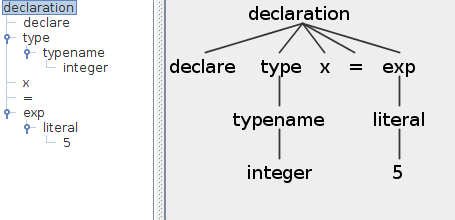
\includegraphics[scale=0.8]{images/pseudo_parse_tree.png}
\caption{Grafički prikaz stabla parsiranja koje generiše parser kreiran od strane \texttt{TestRig} biblioteke za naredbu deklaracije celobrojne promenljive u pseudo-jeziku.}
\label{fig:PseudoTreeGui}
\end{figure}


\subsection{Obilazak stabla parsiranja}
\label{subsec:ANTLRParserIntegration}

ANTLR4, osim leksera i parsera za datu gramatiku, može da kreira interfejse i bazne klase koji prate projektne obrasce \emph{posetilac} (engl. \emph{visitor}) i osluškivač (engl. \emph{listener})\footnote{Osluškivač je varijanta obrasca \emph{posmatrač} (engl. \emph{observer})} opisane u \ref{sec:DesignPatterns}. Tako kreirani interfejsi i klase imaju metode za obilazak stabla parsiranja. ANTLR4 podrazumevano generiše interfejs osluškivača (slika \ref{fig:ANTLRListener}) kao i baznu klasu koja implementira generisani interfejs tako što su sve implementirane metode prazne. Stoga, ukoliko korisnik želi da definiše operaciju samo u slučaju da se prilikom obilaska stabla parsiranja naiđe na određeni tip čvora, nije potrebno implementirati ceo interfejs osluškivača već je moguće naslediti baznu klasu i predefinisati samo jedan metod. ANTLR4 može, pored osluškivača, da generiše i interfejs posetilac (slika \ref{fig:ANTLRVisitor}) ukoliko se navede odgovarajuća opcija \texttt{-visitor} prilikom pokretanja. Slično, ukoliko nije potrebno generisati osluškivač, može se koristiti opcija \texttt{-no-listener}.

\begin{figure}[h!]
\begin{lstlisting}
public interface IPseudoListener : IParseTreeListener
{
    void EnterUnit([NotNull] PseudoParser.UnitContext context);
    void ExitUnit([NotNull] PseudoParser.UnitContext context);
    void EnterBlock([NotNull] PseudoParser.BlockContext context);
    void ExitBlock([NotNull] PseudoParser.BlockContext context);
    void EnterStatement([NotNull] PseudoParser.StatementContext context);
    void ExitStatement([NotNull] PseudoParser.StatementContext context);
    
    ...
}
\end{lstlisting}
\caption{Delimični prikaz interfejsa osluškivača generisanog od strane ANTLR4 za pseudo-jezik definisan u prethodnom odeljku (C\#).}
\label{fig:ANTLRListener}
\end{figure}

Sa slike \ref{fig:ANTLRListener} se vidi da je moguće definisati metode koje će se pozivati prilikom ulaska ali i prilikom izlaska iz čvora određenog tipa prilikom obilaska stabla parsiranja. Pritom je važno kako se stablo obilazi. U slučaju ANTLR4, to je pretraga u dubinu (engl. \emph{depth-first search, DFS})\footnote{DFS je obilazak stabla takav da se obilazak duž grane stabla nastavlja sve dok je moguće ići dublje, a ako to nije moguće vratiti se unazad i obići druge grane.}, stoga će se metod \texttt{Exit} za proizvoljni čvor pozvati tek kad se obiđu sva deca tog čvora --- dakle nakon poziva njihovih \texttt{Enter} i \texttt{Exit} metoda. Pošto se DFS obično implementira putem LIFO strukture\footnote{\emph{Last In, First Out} struktura podataka je apstraktna struktura podataka sa operacijama ubacivanja i izbacivanja elemenata, pri čemu je element koji se izbacuje onaj koji je poslednji ubačen. Primer LIFO strukture je držač za CD-ove --- ne mogu se ukloniti CD-ovi ispod CD-a na vrhu (poslednji ubačen) a da se ne ukloni isti. U slučaju opisanom iznad, implementacija LIFO strukture se naziva stek (engl. \emph{stack}).}, može se reći da se \texttt{Enter} metod poziva onog trenutka kad se čvor ubaci u strukturu, a \texttt{Exit} metod onda kada se čvor ukloni iz strukture.

\begin{figure}[h!]
\begin{lstlisting}
public interface IPseudoVisitor<T> : IParseTreeVisitor<T>
{
    T VisitUnit([NotNull] PseudoParser.UnitContext context);
    T VisitBlock([NotNull] PseudoParser.BlockContext context);
    T VisitStatement([NotNull] PseudoParser.StatementContext context);
    T VisitDeclaration([NotNull] PseudoParser.DeclarationContext context);
    
    ...
}
\end{lstlisting}
\caption{Delimični prikaz interfejsa posetioca generisanog od strane ANTLR4 za pseudo-jezik definisan u prethodnom odeljku (C\#).}
\label{fig:ANTLRVisitor}
\end{figure}

Za razliku od osluškivača, posetilac je prirodnije koristiti ukoliko je potrebno izvršiti neko izračunavanje nad strukturom koja se obilazi. Interfejs posetioca (slika \ref{fig:ANTLRVisitor}) je šablonski, i metodi imaju povratnu vrednost šablonskog tipa za razliku od metoda osluškivača i, u odnosu na osluškivač, nema para metoda za svaki čvor već samo jedan metod. Dodatna razlika, ali i najveća, je ta što se metodi posetioca ne pozivaju automatski. Stoga je na programeru da nastavi obilazak i da odluči u koje čvorove želi da se spusti. Jasno je da i osluškivač i posetilac imaju svoje primene --- ukoliko je potrebno obići stablo parsiranja i dovući neke informacije može se iskoristiti osluškivač jer onda ne moramo brinuti o obilasku. S druge strane, ukoliko je potrebno izračunati neku vrednost prirodno je iskoristiti rekurziju i iskoristiti posetilac --- rekurzivni pozivi prilikom obilaska nam idu u prilog jer koristimo povratne vrednosti tih metoda da gradimo rezultat od listova ka korenu stabla parsiranja. U nastavku će se koristiti posetilac zbog kontrole obilaska ali i činjenice da se stablo parsiranja obilazi sa ciljem da se izgradi AST, koji je takođe rekurzivna struktura i gradi se inkrementalno kroz rekurziju.

Bilo da se koristi osluškivač ili posetilac, potrebno je nekako proslediti informacije o samom čvoru na koji se naišlo tokom obilaska stabla parsiranja. Te informacije se metodima osluškivača i posetioca prosleđuju putem potklasa apstrakne klase konteksta pravila \texttt{ParserRuleContext} --- u primeru iznad \texttt{UnitContext}, \texttt{BlockContext} itd. Svaki kontekst pravila po imenu odgovara pravilima definisanim u gramatici i sadrži informacije bitne za trenutni čvor u stablu parsiranja koji odgovara tipu konteksta. Takođe, u svakom kontekstu su prisutne i metode čija imena odgovaraju pravilima koja se javljaju u definiciji samog pravila koje odgovara kontekstu. Stoga za \texttt{BlockContext}, imajući u vidu definiciju sa slike \ref{fig:PseudoDef1} gde se koristi i pravilo \texttt{statement}, u okviru \texttt{BlockContext} klase biće implementiran i metod \texttt{statement()} koji vraća kontekst pravila tipa \texttt{StatementContext[]}. Metod \texttt{statement()} vraća niz jer u prvoj alternativi stoji \texttt{statement+} --- dakle možemo imati više \texttt{statement} poklapanja. Sa ovim u vidu, moguće je odrediti kako će se obilazak nastaviti (u slučaju posetioca) ili dovući informacije o delovima definicije pravila. Ukoliko pravilo ima više alternativa, metodi koje vraćaju kontekst pravila koje figuriše u alternativi koja nije korišćena za poklapanje pravila će vratiti \texttt{null}. Pošto se \texttt{statement} pravilo javlja u obe alternative pravila \texttt{block} (i nije opciono), možemo biti sigurni da povratna vrednost \texttt{statement()} metoda nikada neće biti \texttt{null}.
